\documentclass[14pt, a4paper]{article}
\usepackage[russian]{babel}
\usepackage{graphicx}
\usepackage{layout}
\usepackage[14pt]{extsizes}
\usepackage{amssymb}
\usepackage{relsize}

\setcounter{tocdepth}{4}
\setcounter{secnumdepth}{4}

\usepackage{xcolor}
\usepackage{hyperref}

\usepackage{listings}

 % Цвета для гиперссылок
\definecolor{linkcolor}{HTML}{000000} % цвет ссылок
\definecolor{urlcolor}{HTML}{000000} %цвет гиперссылок

\hypersetup{pdfstartview=FitH,  linkcolor=linkcolor,urlcolor=urlcolor, colorlinks=true}

\definecolor{codegreen}{rgb}{0,0.6,0}
\definecolor{codegray}{rgb}{0.5,0.5,0.5}
\definecolor{codepurple}{rgb}{0.58,0,0.82}
\definecolor{backcolour}{rgb}{0.97,0.97,0.97}

%таблица
\lstdefinestyle{mystyle}{
    backgroundcolor=\color{backcolour},   
    commentstyle=\color{codegreen},
    keywordstyle=\color{magenta},
    numberstyle=\tiny\color{codegray},
    stringstyle=\color{codepurple},
    basicstyle=\ttfamily\footnotesize,
    breakatwhitespace=false,         
    breaklines=true,                 
    captionpos=b,                    
    keepspaces=true,
    frame=single,                                                    
    showspaces=false,                
    showstringspaces=false,
    showtabs=false,                  
    tabsize=2,
    mathescape=true
}

\lstset{style=mystyle}

%Разметка страницы
\oddsidemargin = 0pt
\marginparwidth = 45pt 
\textwidth = 467pt
\textheight = 716pt
\topmargin = 0pt 
\footskip = 30pt 
\headheight = 0pt 
\headsep = 0pt 

\begin{document}
\begin{titlepage}
    \topmargin=216pt
    \newpage
    \hangindent=0.7cm
    \huge ИУ-10\\
    Системное\\
    Программное\\
    Обеспечение\\
    Администрирование Linux\\
    \textbf{Работа с дисковыми \\
    пространствами. Разделы,\\
    LVM, точки монтирования.}

    \vspace{8cm}

    \begin{center}
        \small\textit{Москва, 2022}
    \end{center}
\end{titlepage}

\section*{На этом уроке} 
\addcontentsline{toc}{section}{На этом уроке}

\begin{enumerate}
    \item Разберем структуру файловой системы
    \item Узнаем, что такое точка монтирования
    \item Познакомимся с понятием раздела, научимся их создавать
    \item Познакомимся с LVM
    \item Выясним, для чего используются ссылки и inode
\end{enumerate}


\tableofcontents
\newpage

\section*{Структура файловой системы} 
\addcontentsline{toc}{section}{Структура файловой системы}

В Linux, так же как и в Windows, физическое хранение данных на диски организуется системой при
помощи файловой системы. А за то, как логически располагаются директории и за их количество
отвечает стандарт иерархии файловой системы (Filesystem Hierarchy Standard). Такую же конструкцию
вы могли видеть в Windows, например, если мы зайдем в директорию диска С: то мы, как минимум
увидим там папки Windows, Program Files, Users и так далее.\\

Дерево каталогов можно посмотреть, используя утилиту \textbf{tree}. Она не идёт в стандартной поставке,
поэтому её необходимо установить, используя команду \colorbox{backcolour}{sudo apt install tree -y}. Утилита
показывает содержимое каталогов в виде дерева. Корневой каталог обозначается точкой. Для
удобства вывода используется параметр \textbf{-d} — показывать только каталоги.

\begin{figure}[h]
    \centering
    \scalebox{0.52}{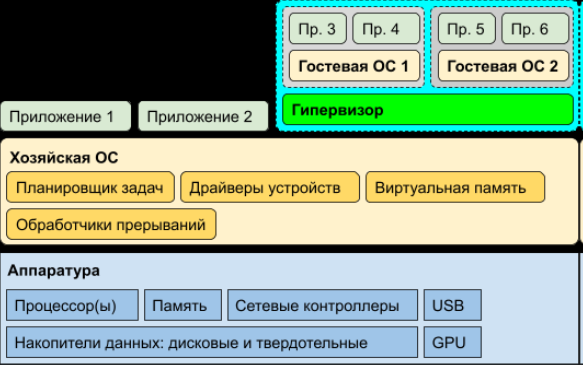
\includegraphics[width=1\textwidth]{1.png}}\\ 
    \small\textit{Рис.1 Структура файловой системы}  
    \label{framework} 
\end{figure}

\newpage

Вложенные каталоги могут быть как самостоятельными единицами файловой системы, хранящими в
себе файлы и другие каталоги, так и точками монтирования для разделов. Разделы либо
организуются на части жёсткого диска, либо занимают всё пространство жесткого диска. На каждом
разделе создаётся собственная файловая система.

\subsection*{Точка монтирования} 
\addcontentsline{toc}{subsection}{Точка монтирования}

В Windows при подключении к ПК правильно отформатированного flash-накопителя или диска
автоматически появляется директория (диск D/E/F), внутри которой будет находится все содержимое
подключенного устройства. Во всех ОС подобная операция называется монтированием, но в Linux у
нее есть свои особенности:

\begin{itemize}
    \item[-] Директория автоматически создана не будет. Необходимо вручную создать папку, в которой
    впоследствии будет находится все содержимое диска или раздела диска. Эта созданная папка
    называется точкой монтирования.
    \item[-] Для доступа к физически подключенному устройству понадобится выполнить команду mount .
    В Windows, к примеру, вручную мы только отключаем флэшку для дальнейшего извлечения из
    ПК. 
\end{itemize}

В результате выполненных действий для конечного пользователя всё будет представляться как
единое пространство данных.

\begin{figure}[h]
    \centering
    \scalebox{0.9}{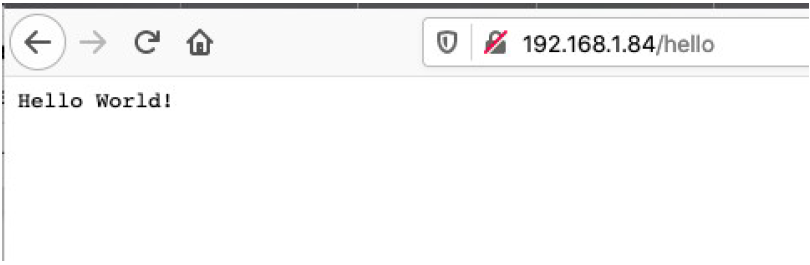
\includegraphics[width=1\textwidth]{2.png}}\\ 
    \small\textit{Рис.2 Блочные устройства в Linux}  
    \label{framework} 
\end{figure}

В файловой системе Linux обычно используется несколько точек монтирования (MOUNTPOINT). С
помощью команды \colorbox{backcolour}{lsblk} можно отобразить все блочные устройства (например, жесткие диски),
используемые в системе. Из рисунка 2 следует, что корневая файловая система находится на одном
устройстве и подключена в точке монтирования \colorbox{backcolour}{“/”} , а в точке \colorbox{backcolour}{/boot} подключено совсем другое
устройство. Схожим образом может осуществляться монтирование и других устройств, в последствии
интегрированных в файловую систему.\\

Чаще всего по разным дискам распределены разные типы данных. Это происходит по следующим
причинам:
\begin{itemize}
    \item Безопасность
\end{itemize}

\noindent Для подключаемого устройства по необходимости могут быть применены более или менее строгие
правила безопасности в зависимости от того, что находится в данном разделе.

\begin{itemize}
    \item Управление
\end{itemize}

\noindent К точке монтирования могут применяться определенные параметры монтирования, которые
необходимы в определенных случаях и не нужны в других.\\

Рассмотрим назначение основных каталогов корневой файловой системы. Обратим внимание, что
многие из них на самом деле являются точками монтирования:

\begin{enumerate}
    \item \textbf{/boot} — каталог, который хранит в себе конфигурационные файлы загрузчика ОС, образы
    ядра и файлы initrd.
    \item \textbf{/bin} и \textbf{/sbin/} — в данных каталогах хранятся основные исполняемые файлы и утилиты,
    необходимые для работы и администрирования операционной системы.
    \item \textbf{/etc} — каталог предназначен для хранения конфигурационных файлов операционной системы
    и всех служб.
    \item \textbf{/home} — стандартный каталог для хранения личных файлов и каталогов пользователей.
    \item \textbf{/dev} — каталог, в котором хранятся файлы устройств (оборудование ПК, которое
    подключается при старте ядра ОС).
    \item \textbf{/proc} — точка монтирования для виртуальной файловой системы procfs, которая используется
    для хранения и предоставления информации о процессах.
    \item \textbf{/sys} — точка монтирования для виртуальной файловой системы sysfs, которая используется
    для хранения и предоставления информации об инициализированных устройствах,
    сгруппированных по разным критериям: типам устройств, шинам, диагностическим протоколам
    доступа и т. п. Одни и те же устройства могут быть показаны в разных каталогах через особый
    тип файлов, который называется символические ссылки, о них поговорим ниже.
    \item \textbf{/usr} — предназначен для хранения пользовательских программ, документации, исходных
    кодов программ и ядра.
    \item \textbf{/var} — каталог содержит в себе постоянно изменяемые файлы, например журналы работы
    операционной системы.
    \item \textbf{/lib} — каталог, который хранит в себе библиотеки и модули ядра, необходимые для
    функционирования ОС.
\end{enumerate}

Команда \colorbox{backcolour}{findmnt} отобразит все точки монтирования, существующие в системе.

\begin{figure}[h]
    \centering
    \scalebox{0.9}{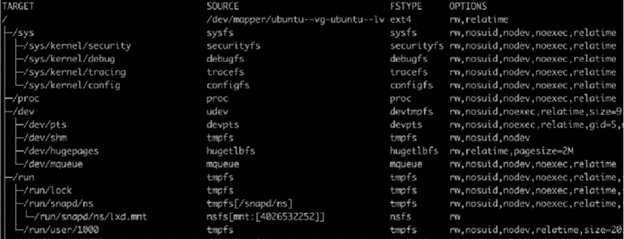
\includegraphics[width=1\textwidth]{3.png}}\\ 
    \small\textit{Рис. 3 Точки монтирования}  
    \label{framework} 
\end{figure}

\section*{Организация хранения} 
\addcontentsline{toc}{section}{Организация хранения}

\subsection*{Структура диска} 
\addcontentsline{toc}{subsection}{Структура диска}

В большинстве случаев к файловой системе подключается не целый диск, а лишь его часть,
называемая разделом или партицией (partition). Основной целью разбиения диска на разделы
является изоляции данных.

\begin{figure}[h]
    \centering
    \scalebox{0.7}{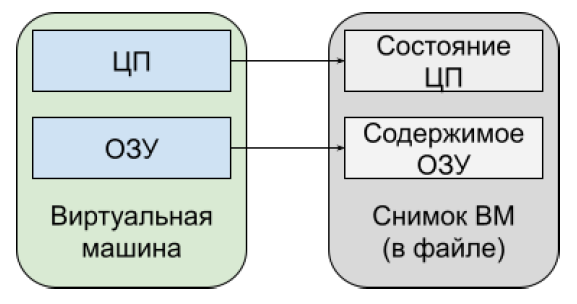
\includegraphics[width=1\textwidth]{4.png}}\\ 
    \small\textit{Рис. 4 Разделы диска}  
    \label{framework} 
\end{figure}

\newpage

На рисунке 4 изображено разделение диска на 4 партиции определенного размера. Для разделов с
первого по третий указанные каталоги будут использоваться в качестве точек монтирования. Таким
образом количество данных внутри этих каталогов не сможет превысить размера партиции, а значит
и влиять на другие данные в системе.

\begin{figure}[h]
    \centering
    \scalebox{0.8}{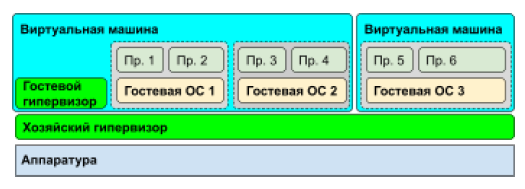
\includegraphics[width=1\textwidth]{5.png}}\\ 
    \small\textit{Рис.5 Имена разделов}  
    \label{framework} 
\end{figure}

Возвращаясь к выводу \colorbox{backcolour}{lsblk}, обратим внимание на тот факт, что диск sda разделен на несколько
разделов (sda1,sda2,sda3). У каждого диска есть имя, которое зависит от типа используемого
устройства. \colorbox{backcolour}{sda} - это имя, которое применяется для первого SCSI-диска в системе, \colorbox{backcolour}{sdb} - для второго
и так далее. В зависимости от имени диска разделы будут названы соответственно.

\subsection*{MBR vs GPT} 
\addcontentsline{toc}{subsection}{MBR vs GPT}

При разбиении диска на разделы возникает два основных вопроса:
\begin{itemize}
    \item[-] Какое количество партиций может существовать?
    \item[-] Какого размера может достигать раздел?
\end{itemize}

В ответе на оба вопроса важную роль играет то, как операционная система загружается. Первым
этапом старта любой ОС, не только Linux, является диагностика оборудования и запуск загрузчика
системы. Загрузчиком может выступать либо BIOS (Basic Input/Output System), либо UEFI (The Unified
Extensible Firmware Interface). BIOS основан на оригинальной спецификации ПК 1981 года и был
изобретен для работы с системами того времени. В те дни, если у компьютера был жесткий диск на
пять мегабайт, он считался большим компьютером. BIOS не был рассчитан на размеры современных
дисков, которые продолжают расти. Вследствие чего в 2010 году появился UEFI. В зависимости от
того, какая система используется для загрузки, используются и разные способы адресации дискового
пространства. Системы BIOS обычно работают с MBR - Master Boot Record, UEFI обычно
поставляются с GPT - GUID Partition Table.

\subsubsection*{MBR} 
\addcontentsline{toc}{subsubsection}{MBR}

\begin{itemize}
    \item[-] Общий размер в 512 байт, что очень мало
    \item[-] 64 байта используется для хранения информации о разделах
    \item[-] Ограничение в 4 раздела размером не более 2 Терабайт
    \item[-] Логические партиции с ограниченной функциональностью могут быть использованы для
    дополнительного разбиения, если не хватает 4
\end{itemize}

\subsubsection*{GPT} 
\addcontentsline{toc}{subsubsection}{GPT}

\begin{itemize}
    \item[-] Больше места для хранения информации о разделах
    \item[-] Используется для преодоления ограничений MBR
    \item[-] 128 разделов, нет необходимости в логических партициях
\end{itemize}

\newpage

\section*{Создание и подключение разделов} 
\addcontentsline{toc}{section}{Создание и подключение разделов}

Для создания разделов существуют несколько утилит.
\begin{itemize}
    \item \colorbox{backcolour}{fdisk} создаст разделы с помощью MBR
    \item \colorbox{backcolour}{gdisk,parted} создадут разделы с помощью GPT
\end{itemize}

Мы будем пользоваться \colorbox{backcolour}{parted} как наиболее современной утилитой для создания GUID разделов.

\subsection*{Создание разделов с помощью parted} 
\addcontentsline{toc}{subsection}{Создание разделов с помощью parted}

Первым шагом необходимо выбрать, на каком диске будут создаваться разделы.

\vspace{0.3cm}

\begin{lstlisting}
root@server:$\sim$# parted /dev/sdb

GNU Parted 3.3

Using /dev/sdb

Welcome to GNU Parted! Type 'help' to view a list of commands.

\end{lstlisting}

\vspace{0.2cm}
Просмотрим и по необходимости создадим таблицу разделов. Следует использовать GPT.
\vspace{0.3cm}

\begin{lstlisting}
(parted) print

Error: /dev/sdb: unrecognised disk label

Model: ATA VBOX HARDDISK (scsi)

Disk /dev/sdb: 1074MB

Sector size (logical/physical): 512B/512B

Partition Table: unknown

Disk Flags:

(parted) mklabel gpt

(parted) print

Model: ATA VBOX HARDDISK (scsi)

Disk /dev/sdb: 1074MB

Sector size (logical/physical): 512B/512B

Partition Table: gpt

Disk Flags:

Number Start End Size File system Name Flags

\end{lstlisting}

\vspace{0.2cm}
При наличии таблицы можно переходить к созданию самих разделов с помощью команды \colorbox{backcolour}{mkpart}.
\vspace{0.3cm}

\begin{lstlisting}
(parted) mkpart

Partition name? []? database

File system type? [ext2]?

Start? 0

End? 100

Warning: The resulting partition is not properly aligned for best 
performance: 34s % 2048s != 0s

Ignore/Cancel?

Ignore/Cancel? Ignore

(parted)

(parted) print

Model: ATA VBOX HARDDISK (scsi)

Disk /dev/sdb: 1074MB

Sector size (logical/physical): 512B/512B

Partition Table: gpt

Disk Flags:

Number Start   End    Size  File system Name      Flag

 1     17.4kB 100MB  100MB  ext2         databas

\end{lstlisting}

\vspace{0.2cm}

\textbf{Важно!} \underline{\textit{Start/End \ - \ начало/окончание раздела отсчитываются от}} \\
\underline{\makebox[\linewidth][s]{\textit{начала диска и по умолчанию считается в Мегабайтах. При создании}}} \\
\underline{\textit{второго раздела сразу после приведенного в пример Start необходимо ука-}} \\
\underline{\textit{зывать - 100, End - 100 + необходимый размер партиции.}}\\

После создания всех необходимых разделов выходим из утилиты и выполняем \colorbox{backcolour}{udevadm settle},
чтобы убедиться, что устройство было создано. 
\newpage 

\begin{lstlisting}
(parted)quit

root@server:$\sim$# udevadm settle

root@server:$\sim$# lsblk

sdb                          8:16    0     1G  0  disk
 $ {^\mathlarger{\mathlarger{{\mathlarger{\llcorner}}}}} $sdb                        8:17    0  95.4M  0  part
\end{lstlisting}

\vspace{0.2cm}

При создании раздела вы не создаете файловую систему, как это часто делают другие операционные
системы. В \colorbox{backcolour}{parted} есть атрибут файловой системы, но этот атрибут можно игнорировать, так как он
записывает только некоторые незначительные метаданные файловой системы.

\subsection*{Создание файловой системы} 
\addcontentsline{toc}{subsection}{Создание файловой системы}

После создания раздела нужно установить файловую систему поверх него. Файловая система
определяет метод, который используется для записи данных на диск, организации этих данных в
блоки, а также выполнения всех остальных действий, связанных с хранением информации на диске.
Существуют два основных типа файловых систем: XFS и ext4.

\subsubsection*{XFS} 
\addcontentsline{toc}{subsubsection}{XFS}

\begin{itemize}
    \item[-] Быстрая и масштабируемая
    \item[-] Использует технологию записи CoW (Copy on Write) для гарантии целостности файлов.
    Перед записью изменения на диск исходный файл копируется в другое место для
    возможности возврата к предыдущему состоянию файла.
    \item[-] Существует возможность увеличения размеров файловой системы, но не уменьшения
\end{itemize}

\subsubsection*{Ext4} 
\addcontentsline{toc}{subsubsection}{Ext4}

\begin{itemize}
    \item[-] Для гарантии целостности файлов используется журналирование. При любой записи в файл
    журнал отслеживает изменения, и, если что-то пойдет не так, на основе информации в
    журнале легко вернуться к предыдущему состоянию файла
    \item[-] Существует возможность как увеличения так и уменьшения размеров файловой системы
    \item[-] Обратно совместима с устаревшей ext2
    \item[-] Архитектура файловой системы основана на подходе к хранению данных, который более не
    используется  
\end{itemize}

Существуют и другие файловые системы (btrfs,zfs), но они менее распространены.\\

\textbf{Примечание!} \underline{\textit{Так как для каждого раздела создается своя файловая}}\\
\underline{\textit{система, то для нескольких разделов можно использовать разные фай-}} \\
\underline{\textit{ловые системы. На одном может xfs, на втором - ext4, на третьем - }}\\
\underline{\textit{zfs и тд. Все эти файловые системы будут нормально сосуществовать}} \\
\underline{\textit{внутри одной ОС}}.\\

Создание файловых систем в других операционных системах известно как форматирование раздела
или диска. В Linux предпочтительна терминология именно создания, так как для этого используется
утилита \colorbox{backcolour}{mkfs}. Для \colorbox{backcolour}{xfs} используется команда \colorbox{backcolour}{mkfs.xfs} и \colorbox{backcolour}{mkfs.ext4} - для ext4 соответственно.

\vspace{0.3cm}

\begin{lstlisting}
root@server:$\sim$# mkfs.xfs /dev/sdb1

meta-data=/dev/sdb1                           agcount=4, agsize=6103 blks

         =                       sectsz=512   attr=2,

         =                       crc=         finobt=1, sparse=1,

         =                       reflink=

data     =                       bsize=4096   blocks=24409,

         =                       sunit=       swidth=0 blks

naming   =version 2              bsize=4096   ascii-ci=0,

log      =internal log           bsize=4096   blocks=1368,

         =                       sectsz=512   sunit=0 blks, lazy-
         
realtime                         extsz=4096   blocks=0,

$$

\end{lstlisting}

\vspace{0.3cm}

\textbf{Важно!} \underline{\textit{Не используйте mkfs без каких-либо экстеншенов (xfs,ext4),}} \\
\underline{\makebox[\linewidth][s]{\textit{так как в этом случае будет создана устаревшая файловая система}}} \\
\underline{\textit{Ext2.}}

\newpage

\subsection*{Монтирование файловой системы} 
\addcontentsline{toc}{subsection}{Монтирование файловой системы}

Последним шагом является непосредственно монтирование созданной файловой системы в точке
монтирования. Эта операция выполняется с помощью команды \colorbox{backcolour}{mount <файловая система>
<точка монтирования>}.

\vspace{0.3cm}

\begin{lstlisting}
root@server:$\sim$# mkdir /opt/database

root@server:$\sim$# du -sh /opt/database/

4.0K /opt/database/

root@server:$\sim$# mount /dev/sdb1
/opt/database/


$\vdash$/opt/database                      /dev/sdb                        xfs
rw,relatime,attr2,inode64,logbufs=8,logbsize=32k,noquota

root@server:$\sim$# du -sh /opt/database/

0 /opt/database/
$$
\end{lstlisting}
\vspace{0.2cm}

Теперь на на данный раздел диска с файловой системой можно записывать данные, а с помощью
команды \colorbox{backcolour}{umount <точка монтирования>} выполнить операцию отключения раздела от точки
монтирования.

\vspace{0.3cm}
\begin{lstlisting}
root@server:$\sim$# mount /dev/sdb1 /opt/database/

root@server:$\sim$# cat /var/log/syslog > /opt/database/some_data

root@server:$\sim$# du -sh /opt/database/

16K /opt/database/

root@server:$\sim$# ls -l

/opt/database/ total 4

-rw-r--r-- 1 root root 20 Jan 7 17:21 some_data

root@server:$\sim$# umount /opt/database

root@server:$\sim$# du -sh /opt/database/

4.0K /opt/database/

root@server:$\sim$# ls -l

/opt/database/ total 0
$$
\end{lstlisting}
\vspace{0.2cm}

При помощи команды \colorbox{backcolour}{mount} без каких-либо ключей можно увидеть примонтированные файловые
системы.

\begin{lstlisting}
root@server:$\sim$# mount

sysfs on /sys type sysfs (rw,nosuid,nodev,noexec,relatime)

proc on /proc type proc (rw,nosuid,nodev,noexec,relatime)

/dev/mapper/ubuntu--vg-ubuntu--lv on / type ext4 (rw,relatime)

tmpfs on /dev/shm type tmpfs (rw,nosuid,nodev)

tmpfs on /run/lock type tmpfs (rw,nosuid,nodev,noexec,relatime,size=5120k)

tmpfs on /sys/fs/cgroup type tmpfs (ro,nosuid,nodev,noexec,mode=755)

...
$$
\end{lstlisting}

\vspace{0.2cm}

\textbf{Важно!} \underline{\textit{При перезагрузке системы все файловые системы будут ав-}} \\
\underline{\textit{томатически размонтированы}}.

\subsubsection*{Автоматическое монтирование} 
\addcontentsline{toc}{subsubsection}{Автоматическое монтирование}

Монтирование разделов в точки монтирования при старте операционной системы организуется через
специальный файл \textbf{/etc/fstab}, в котором прописываются имя устройства, тип файловой системы,
точка монтирования и дополнительные опции монтирования.

\begin{figure}[h]
    \centering
    \scalebox{1}{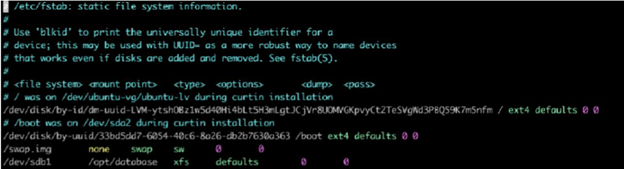
\includegraphics[width=1\textwidth]{6.png}}\\ 
    \small\textit{Рис 6. Содержание /etc/fstab}  
    \label{framework} 
\end{figure}

На рисунке 6 в последней строке описаны инструкции для монтирования созданной ранее файловой
системы. Разберем ее по порядку:

\begin{itemize}
    \item[-] /dev/sdb1 - ранее созданный раздел диска с файловой системой
    \item[-] /opt/database - точка монтирования
    \item[-] xfs - тип используемой файловой системы
    \item[-] defaults - опции, связанные с файловой системой. К примеру файловую систему можно
    примонтировать в режиме read only
    \item[-] Последние два нуля связаны с отключением использования утилит dump и fsck.
\end{itemize}

Файловые системы будут автоматически примонтированы при старте, либо можно воспользоваться
командой \colorbox{backcolour}{mount -a}. Более подробно о утилитах mount, umount, а также файле /etc/fstab можно
прочитать на соответствующих страницах встроенного справочного руководства man.\\

\textbf{Важно!} \underline{\textit{Необходимо  быть \ крайне \ внимательным \ при \ заполнении}}\\ 
\underline{\textit{/etc/fstab, \ так как в случае \ ошибок и опечаток \ операционная система}} \\
\underline{\textit{загрузится в rescue mode, то есть с ограниченным функционалом и бу-}} \\
\underline{\textit{дет доступна только через терминал сервера или виртуальной машины}}.

\newpage

\subsection*{Расширенные возможности хранения данных} 
\addcontentsline{toc}{subsection}{Расширенные возможности хранения данных}

Если использовать традиционные разделы, которые обсуждались ранее в уроке, мы столкнемся с
набором ограничений:

\begin{itemize}
    \item[-] без остановки системы разделы невозможно переразбить или заменить.
    \item[-] отсутствует возможность начать работать с двумя дисками как с одним разделом.
    Можно смонтировать разные разделы и диски в одну виртуальную файловую систему. У вас
    могут быть /home, /bin, /usr/bin и т.д. — все на разных дисках (когда-то так и было). Но это не
    позволит, например, увеличить в два раза дисковое пространство под /home без остановки
    системы и замены диска/раздела.
\end{itemize}

\noindent Для решения описанных проблем можно использовать LVM (Logical Volume Manager), Stratis, или VDO
(Virtual Data Optimizer). LVM существует уже довольно давно, широко распространен и используется
по умолчанию при установке Ubuntu, поэтому мы подробнее остановимся именно на нем.

\begin{figure}[h]
    \centering
    \scalebox{0.6}{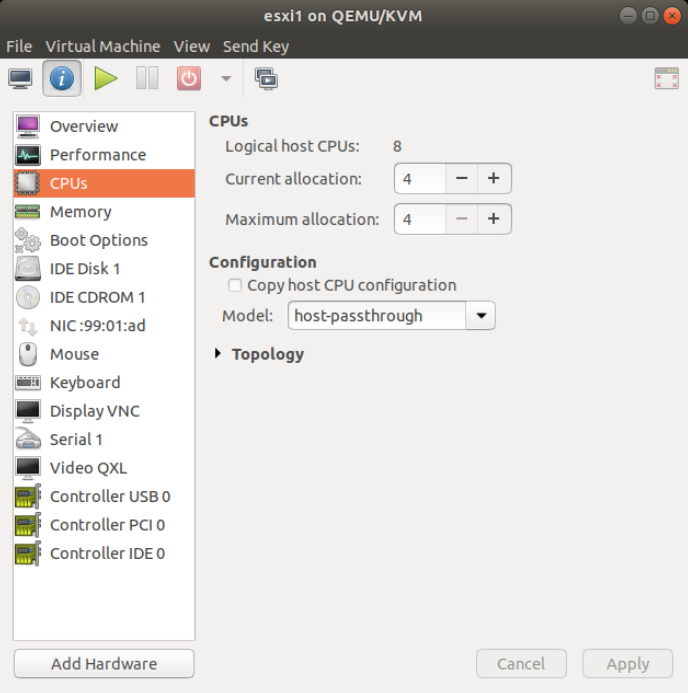
\includegraphics[width=1\textwidth]{7.png}}\\ 
    \small\textit{Рис.7 Структура LVM}  
    \label{framework} 
\end{figure}

На рисунке 7 изображена структура LVM. Центральным элементом является группа томов или Volume
Group. Volume Group - это объединение устройств хранения информации, доступных в системе, в
единое целое. Важно отметить, что эти устройства хранения могут быть чем угодно: дисками,
разделами, LUN в SAN - все они представляются в виде абстракции, называемой физическим томом
(Physical Volume - PV). Таким образом, если у нас есть 4 диска по 500Гб, мы можем преобразовать
каждый в физический том (на рисунке PV1-4) и объединить в группу, получив 2Тб доступного места.\\

Полученные 2Тб можно разделить на логические тома (Logical Volume - LV). Эти логические тома
используются аналогично стандартным разделам диска, то есть поверх них создаются свои файловые
системы, которые впоследствии будут смонтированы в точках монтирования (на рисунке 
\textbf{//usr/home/opt/var/home}).\\

В частном случае можно все свободное место в группе отдать под один логический том, тем самым
получив виртуальный диск на 2Тб.\\

LVM хорош по нескольким причинам:
\begin{itemize}
    \item[-] LVM предлагает гибкое решение для управления хранилищем. Объемы больше не привязаны
    к ограничениям физических жестких дисков (LV2 на рисунке 7). Если требуется
    дополнительное пространство для хранения, группу томов можно легко расширить, добавив
    новый физический том, чтобы можно было добавить дисковое пространство к логическим
    томам.
    \item[-] Поддержка snapshot. snapshot сохраняет текущее состояние логического тома и может
    использоваться для отката изменений или создания резервной копии файловой системы.
    \item[-] возможность простой замены вышедшего из строя оборудования. Если жесткий диск выходит
    из строя, данные могут быть перемещены внутри группы томов с помощью команды pvmove,
    отказавший диск затем может быть удален из группы томов, а новый жесткий диск может быть
    добавлен динамически, без простоя.
\end{itemize}

\subsection*{Работа с LVM} 
\addcontentsline{toc}{subsection}{Работа с LVM}

\subsubsection*{Создание логических томов} 
\addcontentsline{toc}{subsubsection}{Создание логических томов}

Давайте пошагово разберем, как можно взаимодействовать с Logical Volume Manager.\\

LVM может работать с целыми устройствами, но рекомендуется использовать разделы, потому что это
упрощает распознавание того, что происходит на устройствах в настройке LVM, так что сначала нужно
создать раздел. В parted потребуется установить лейбл \colorbox{backcolour}{lvm on}.

\vspace{0.3cm}

\begin{lstlisting}
(parted) mkpart

Partition name? []? lvm_part

File system type? [ext2]?

Start? 100

End? 200

Warning: The resulting partition is not properly aligned for best 
performance: 195313s % 2048s != 0s

Ignore/Cancel? Ignore

(parted) print

Model: ATA VBOX HARDDISK (scsi)

Disk /dev/sdb: 1074MB

Sector size (logical/physical): 512B/512B

Partition Table: gpt

Disk Flags:

Number Start    End   Size    File system Name       Flags

 1      17.4kB 100MB 100MB   xfs           database

 2      100MB  200MB 100MB   ext2          lvm_part

(parted) set 2 lvm on

(parted) print

Model: ATA VBOX HARDDISK (scsi)

Disk /dev/sdb: 1074MB

Sector size (logical/physical): 512B/512B

Partition Table: gpt

Disk Flags:

Number Start    End   Size    File system Name       Flags

 1     17.4kB   100MB 100MB  xfs           database

 2     100MB    200MB 100MB  ext2          lvm_part  lvm

\end{lstlisting}

\newpage

Создадим из раздела Physical Volume или физический том.
\vspace{0.3cm}

\begin{lstlisting}
root@server:$\sim$# pvcreate /dev/sdb2

  Physical volume "/dev/sdb2" successfully created.

root@server:$\sim$# pvs

  PV         VG        Fmt Attr

  /dev/sda3  ubuntu-vg lvm2 a--              0

  /dev/sdb             lvm2 --- <95.37m <95.37m
$$
\end{lstlisting}
\vspace{0.2cm}

Создадим новую Volume Group и добавим в нее созданный ранее физический том. Все это можно
сделать с помощью одной команды. Последующее расширение группы выполняется с помощью
\colorbox{backcolour}{vgextend}.

\vspace{0.3cm}

\begin{lstlisting}
root@server:$\sim$# vgcreate example_vg
  
  /dev/sdb2 Volume group "example_vg"
  
  successfully created

  VG        #PV #LV #SN Attr   VSize VFree

  exampl      1   0   0 wz--n- 92.00m

  ubuntu-vg   1   1   0 wz--n-            0
  $$
\end{lstlisting}
\vspace{0.2cm}

Теперь можем выделить часть группы под логический том.
\vspace{0.3cm}

\begin{lstlisting}
root@server:$\sim$# lvcreate -n example_lv -L 20M

root@server:$\sim$# lvcreate -n example_lv -L 20M

example_vg

  Logical volume "example lv" created.

   LV         VG       Attr       LSize Pool Origin Data% Meta% Move Log
 Cpy%Sync Convert

  example_lv          example_vg
            -wi-a-----
$$
\end{lstlisting}
\vspace{0.2cm}

С помощью опции -n можно задать имя, а -L - размер тома. \\

\textbf{Примечание!} \underbar{\textit{Если имя не задано, то ОС сгенерирует сама и оно бу-}} 
\\ \underbar{\textit{дет не очевидно}}.\\

Создаем и монтируем файловую систему по аналогии с обычным разделом.
\vspace{0.3cm}

\begin{lstlisting}
root@server:$\sim$# mkfs.xfs /dev/example_vg/example_lv

meta-data=/dev/example_vg/example_lv                isize=512 agcount=1,

         =                       sectsz=512         attr=2,

         =                       crc=               finobt=1, sparse=1,

         =                       reflink=

data     =                       bsize=4096         blocks=5120,

         =                       sunit=             swidth=0 blks

naming   =version 2              bsize=4096         ascii-ci=0, ftype=1

log      =internal log           bsize=4096         blocks=1368,

         =                       sectsz=512         sunit=0 blks, lazy-
         
realtime                         extsz=4096         blocks=0,

root@server:$\sim$# mkdir /opt/example_lvm

root@server:$\sim$# mount

/dev/example_vg/example_lv /opt/ database/

example_lvm/
$$
\end{lstlisting}

\subsubsection*{Увеличение логических томов} 
\addcontentsline{toc}{subsubsection}{Увеличение логических томов}

Для создания логического тома было использовано не все пространство, доступное в созданной
Volume Group.
\vspace{0.3cm}

\begin{lstlisting}
root@server:$\sim$# vgs

  VG      #PV #LV #SN Attr   VSize  VFree

  exampl   1   1   0  wz--n- 92.00m 72.00m

root@server:$\sim$# lvs

  LV         VG        Attr        LSize Pool Origin Data% Meta% Move Log

Cpy%Sync

  example_lv        example_vg    -wi-ao---- 20.00m

\end{lstlisting}
\vspace{0.2cm}

Для увеличения логического тома следует воспользоваться утилитой \colorbox{backcolour}{lvextend}.

\newpage

\begin{lstlisting}

root@server:$\sim$# lvextend -r -L +72M /dev/

/dev/example_vg/example_lv  /dev/ubuntu-vg/ubuntu-lv

root@server:$\sim$# lvextend -r -L +72M

/dev/example_vg/example_lv

  Size of logical volume example_vg/example_lv changed from 20.00 MiB 
  (5 extents) to 92.00 MiB (23 extents).

  Logical volume example_vg/example_lv successfully resized.

meta-data=/dev/mapper/example_vg-example_lv isize=512 agcount=1, agsize=5120 blks

         =                       sectsz=512   attr=2, projid32bit=1

         =                       crc=1        finobt=1, sparse=1, rmapbt=0

         =                       reflink=1

data     =                       bsize=4096   blocks=5120, imaxpct=25

         =                       sunit=0      swidth=0 blks

naming   =version 2              bsize=4096   ascii-ci=0, ftype=1

log      =internal log           bsize=4096   blocks=1368, version=2

         =                       sectsz=512   sunit=0 blks, lazy-count=1

realtime =none                   extsz=4096   blocks=0, rtextents=0

data blocks changed from 5120 to 23552

root@server:$\sim$# vgs

  VG          #PV #LV #SN Attr    VSize VFree

  example_vg        1  1          0 wz--n-

  92.00m      0

  ubuntu-vg     1   1  0   wz--n- <9.00g   0

root@server:$\sim$# lvs

  LV          VG         Attr        LSize Pool Origin Data% Meta% Move Log
Cpy%Sync Convert

  example_lv           example_vg    -
$$
\end{lstlisting}
\vspace{0.2cm}

Помимо изменения размеров логического тома, требуется изменить и размер файловой системы,
установленной на него. Для этого следуют вос- 
\makebox[\linewidth][s]{пользоваться утилитами \colorbox{backcolour}{e2resize,xfs\_growfs} или ключом -r в утилите} 
\colorbox{backcolour}{lvextend}. С помощью ключа -L указываем, на сколько нужно увеличить размер
логического тома.\\

Исходя из выводов, все свободное пространство в группе было использовано. Для дальнейшего
расширения логического тома или создания нового понадобится создать новый физический том и
добавить его в группу example\_vg с помощью команды \colorbox{backcolour}{vgextend}.

\section*{Мониторинг доступного места} 
\addcontentsline{toc}{section}{Мониторинг доступного места}

Для нахождения количества свободного места существуют две утилиты: \colorbox{backcolour}{df,du}. Отличие этих утилиты
заключается в том, откуда они берут информацию о доступном пространстве. \colorbox{backcolour}{df} запрашивает
информацию из установленной файловой системы, \colorbox{backcolour}{du} в свою очередь опирается на данные
непосредственно с диска. Бывают случаи, когда данные от утилит разнятся.\\

В обеих утилитах полезным ключом является -h или - -human-readable. Без него информация будет
отражена в блоках.
\vspace{0.3cm}

\begin{lstlisting}
root@server:$\sim$# df -h

Filesystem                          Size  Used Avail Use% Mounted on

udev                                951M     0  951M   0% /dev

tmpfs                               199M    1M  198M   1% /run

/dev/mapper/ubuntu--vg-ubuntu--lv   8.8G  4.6G  3.8G  55% /
                                            
tmpfs                               994M     0  994M   0% /dev/shm

tmpfs                               5.0M     0  5.0M   0% /run/lock
                                            
tmpfs                               994M     0  994M   0% /sys/fs/cgroup
                                            
/dev/sda2                           976M  264M  712M  22% /boot
                                            
/dev/loop0                          56M    56M     0 100% /snap/core18/1932
                                            
/dev/loop1                          56M    56M     0 100% /snap/core18/1944
                                           
/dev/loop2                          72M    72M     0 100% /snap/lxd/16099
                                            
/dev/loop3                          68M    68M     0 100% /snap/lxd/18150

/dev/loop4                          32M    32M     0 100% /snap/snapd/10492

tmpfs                               199M     0  199M   0% /run/user/1000

/dev/loop6                          32M    32M     0 100% /snap/snapd/10707

/dev/mapper/example                 87M   2.0M   85M   3%
$$
\end{lstlisting}
\vspace{0.2cm}

Утилита du требует указания пути до каталога.
\vspace{0.3cm}

\begin{lstlisting}
root@server:$\sim$# du -h

/opt/database/ 16K
$$
\end{lstlisting}

\subsection*{Ссылки и файловые дескрипторы} 
\addcontentsline{toc}{subsection}{Ссылки и файловые дескрипторы}

Для сохранения свободного места можно воспользоваться концепцией ссылок. Ссылки — это
особенность файловой системы, которая позволяет размещать один и тот же файл в разных
каталогах.\\

Перед тем, как воспользоваться ссылками, следует познакомиться с понятием индексного
дескриптора. С каждым файлом в операционной системе Linux связана особая структура данных —
индексный дескриптор (\textbf{inode}). Эти данные хранят метаинформацию о файле: владелец, права
доступа, время последнего изменения и т. д. Inode также содержит информацию о физическом
расположении данных.\\

Inode уникальны на уровне разделов. Вы можете иметь два файла с одинаковым номером inode, если
они находятся в разных разделах. Информация inode хранится в табличном формате в виде
структуры в начале каждого раздела. Просмотреть inode можно, используя команду \textbf{ls -li}.

\vspace{0.3cm}

\begin{lstlisting}
# ls -li

$\mathbf{434234}$ drw-r--r-- 2 root            examples 4096 Dec 1 14:27 dir

$\mathbf{434231}$ drw-rwSr-t 2 root            developers 4096 Dec 1 14:52 dir1

$\mathbf{434232}$ drw-rw-rwT 2 root            root       4096 Dec 1 14:53 dir2

$\mathbf{422147}$ -rwsr-xr-x 1 root root           0 Dec 1 14:04 myfile

\end{lstlisting}

\vspace{0.2cm}

Каталог содержит таблицу соответствия \textbf{имя\_файла} → \textbf{inode}. В этой таблице требуется уникальность
имён, но не уникальность номеров inode. Благодаря этому каждый объект файловой системы может
иметь несколько имён.\\

Вернемся к ссылкам. \textbf{Жёсткая ссылка} — это запись в каталоге, указывающая на inode. Жёсткая
ссылка создаётся только для файлов, за исключением специальных записей, указывающих на саму
директорию (.) и родительскую директорию (..). Жёсткие ссылки используются только в пределах
одного раздела. На практике жёсткие ссылки уже почти не применяются в работе. Создать жёсткую
ссылку можно, используя команду \textbf{ln} без параметров, например \colorbox{backcolour}{ln file link}, 
где \colorbox{backcolour}{file} — имя файла-источника, \colorbox{backcolour}{link} — имя ссылки на файл. Родительский файл можно перемещать или даже
удалять без вреда для ссылки, то есть фактически файл, на который есть хотя бы одна жёсткая
ссылка, не перестанет существовать. Изменение содержимого файла и разрешений также повлияет и
на ссылку.\\

\href{https://ru.wikipedia.org/wiki/Символическая_ссылка}{\textbf{Символическая ссылка}} — это запись в каталоге, указывающая на имя объекта с другим inode.
Символическая ссылка наиболее близка к ярлыку в Windows. Символическая ссылка может
ссылаться на файл и на каталог. Символические ссылки могут существовать на разных разделах.
Права доступа и inode у символической ссылки отличаются от родительского файла. При
перемещении или удалении файла-родителя символическая ссылка «ломается», так как ссылка
привязывается именно к имени файла. Создать символическую ссылку можно командой \colorbox{backcolour}{ln -s file
link}, где параметр \textbf{-s} говорит, что мы создаём символическую ссылку, \colorbox{backcolour}{file} — имя источника файла,
\colorbox{backcolour}{link} — имя ссылки на файл.

\begin{figure}[h]
    \centering
    \scalebox{0.9}{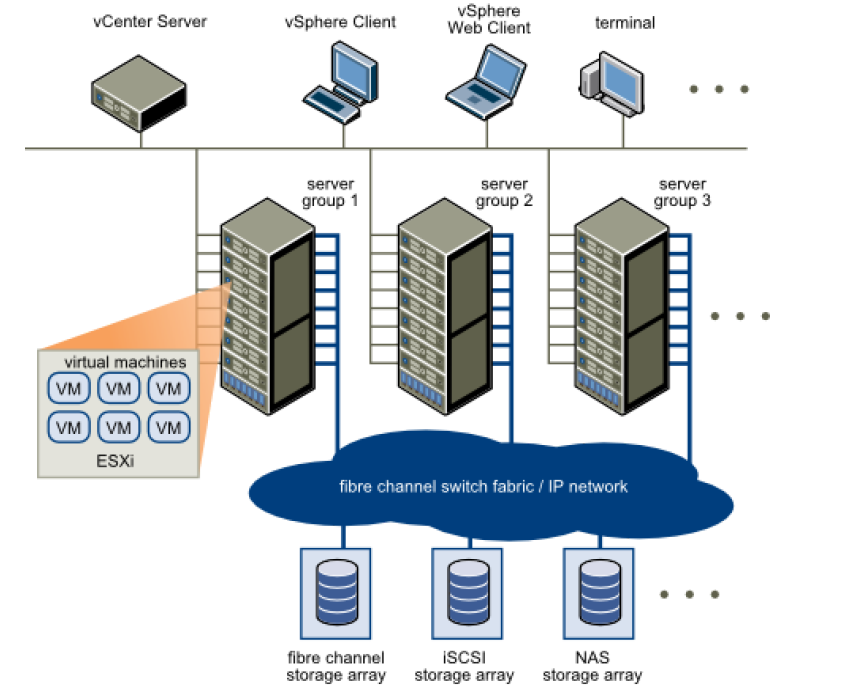
\includegraphics[width=1\textwidth]{8.png}}\\ 
    \small\textit{Рис. 9 Ссылки и дескрипторы}  
    \label{framework} 
\end{figure}

\newpage

\section*{Практическое задание} 
\addcontentsline{toc}{section}{Практическое задание}

\textbf{Внимание!} \underbar{\textit{Перед началом выполнения работы рекомендуется сделать}} \\
\underbar{\textit{snapshot виртуальной машины, чтобы можно было откатить измене-}} \\
\underbar{\textit{ния в случае ошибок. Размер добавляемого диска и создаваемых разделов}} \\
\underbar{\textit{дозволяется варьировать, в зависимости от возможностей ПК}}.

\begin{enumerate}
    \item Добавить к серверу второй жесткий диск размером 300 Мегабайт
    \begin{enumerate}
        \item[a.] Разбить диск на 2 раздела по 150 Мб
        \item[b.] На первом разделе создать файловую систему Ext4 и примонтировать к папке
        /mnt/ext4
        \item[c.] Добавить точку монтирования \textbf{/mnt/ext4} в \textbf{/etc/fstab}
    \end{enumerate}
    \item На втором разделе создать локальный том (LVM) размером 100 Мб. Создать файловую
    систему XFS и примонтировать к папке \textbf{/mnt/xfs}.
    \item Создать файл \textbf{/mnt/ext4/file1} и наполнить его произвольным содержимым. Скопировать его в
    file2. Создать символическую ссылку file3 на file1. Создать жёсткую ссылку file4 на file1.
    Посмотреть, какие inode у файлов. Удалить file1. Что стало с остальными созданными
    файлами? Попробовать вывести их на экран.
    \item Создать ссылку вида \textbf{/mnt/xfs/link}, по которой будет доступен \textbf{/mnt/ \\ ext4/file4}.
\end{enumerate}

\section*{Глоссарий} 
\addcontentsline{toc}{section}{Глоссарий}

\href{https://help.ubuntu.ru/wiki/разделы_и_файловые_системы_linux}{\underbar{\textbf{Раздел}}} — часть долговременной памяти жёсткого диска или флеш-нако- 
пителя, выделенная для удобства работы и состоящая из смежных блоков. 
На одном устройстве хранения может быть несколько разделов.\\

\noindent \href{https://ru.wikipedia.org/wiki/Точка_монтирования}{\underbar{\textbf{Точка монтирования}}} — это каталог, с помощью которого обеспечивается доступ к новой файловой
системе, каталогу или файлу. Точка монтирования используется для реализации возможности
динамически присоединять разделы диска к файловой системе и отсоединять их во время работы
операционной системы.\\

\noindent \href{https://opencentr.ru/article/fajlovaya-sistema-linux/}{\underbar{\textbf{Файловая система}}} — часть операционной системы, которая обеспечивает чтение и запись файлов
на дисковых носителях информации. Файловая система устанавливает физическую и логическую
структуру файлов, правила их создания и управления ими, а также сопутствующие данные файла и
идентификацию. Конкретная файловая система определяет размер имени файла и максимально
возможный размер файла.\\

\noindent \href{https://help.ubuntu.ru/wiki/lvm}{\underbar{\textbf{Logical Volume Manager (LVM)}}} — система управления томами с данными для Linux. Она позволяет
создавать поверх физических разделов (или даже неразбитых жёстких дисков) логические тома,
которые в самой системе будут видны как обычные блочные устройства с данными, то есть как
обычные разделы.\\

\noindent \href{https://ru.wikipedia.org/wiki/Inode}{\underbar{\textbf{Inode}}} — индексный дескриптор, структура данных в файловых системах Linux. Предназначена для
хранения метаинформации о стандартных файлах, каталогах или других объектах файловой
системы, кроме непосредственно данных и имени.

\section*{Дополнительные материалы} 
\addcontentsline{toc}{section}{Дополнительные материалы}

\href{https://losst.ru/tipy-fajlovyh-sistem-dlya-linux}{\textit{Типы файловых систем Linux}}\\

\noindent \href{http://parallel.uran.ru/book/export/html/382}{\textit{inode и каталоги}}

\section*{Используемые источники} 
\addcontentsline{toc}{section}{Используемые источники}

\href{https://it.wikireading.ru/6453}{\textit{Робачевский Андрей М. Операционная система Unix}}\\

\noindent \href{https://www.linuxcenter.ru/lib/books/kostromin}{\textit{В.Костромин, "Linux для пользователя",изд."БХВ-Петербург", 2002 г., серия "Самоучитель"}}\\

\noindent \href{https://habr.com/ru/post/67283/}{\textit{LVM - это просто!}}

\end{document}